\documentclass[10pt]{article}
\usepackage[margin=1in, paperwidth=8.5in, paperheight=11in]{geometry}
\usepackage{ifpdf,amsmath, amssymb, comment, color, graphicx, stmaryrd,setspace,enumitem,tikz, fancyhdr, wrapfig, textcomp, units, mathptmx, pdfpages, cancel, multicol}
\usepackage{hyperref}
\hypersetup{
    colorlinks=true,
    urlcolor=blue,
}

\setlength{\headheight}{14.5pt}
\newcommand{\Q}{\mathbb{Q}}
\newcommand{\R}{\mathbb{R}}
\newcommand{\Z}{\mathbb{Z}}
\newcommand{\vu}{\mathbf{u}}
\newcommand{\vv}{\mathbf{v}}
\newcommand{\vw}{\mathbf{w}}
\newcommand{\vi}{\mathbf{i}}
\newcommand{\vj}{\mathbf{j}}
\newcommand{\vk}{\mathbf{k}}
\newcommand{\vn}{\mathbf{n}}
\newcommand{\vr}{\mathbf{r}}
\newcommand{\va}{\mathbf{a}}
\newcommand{\vF}{\mathbf{F}}
\newcommand{\vL}{\mathbf{L}}
\newcommand{\vT}{\mathbf{T}}
\newcommand{\vN}{\mathbf{N}}
\newcommand{\proj}{\operatorname{proj}}
\newcommand{\orth}{\operatorname{orth}}
\newcommand\del\nabla
\newcommand\dotp[1][.5]{\,\mathbin{\vcenter{\hbox{\scalebox{#1}{$\bullet$}}}}\,}
\newcommand{\slice}{_\text{slice}}

% Solution text is in red. If you want the solutions to show, remove the \iffalse from the definition of the \red command.
%\newcommand{\red}[1]{ %\iffalse
%	\textcolor{red}{#1} }%\fi}

\newenvironment{red}{\color{red}}{\ignorespacesafterend}
\newenvironment{blue}{\color{blue}}{\ignorespacesafterend}
\newcommand{\green}[1]{\textcolor{green}{#1}}
\renewcommand{\section}[1]{\begin{center} \textbf{#1} \\\end{center}}
%
\hyphenpenalty=5000
\setlength{\parindent}{0in}
%\oddsidemargin=-.25in
\allowdisplaybreaks
\pagestyle{fancy}
\renewcommand{\headrulewidth}{0pt}
\lhead{MATH 202}
\rhead{Spring 2024}
%\lfoot{\copyright\ CLEAR Calculus 2010}
\cfoot{}

\begin{document}
%


%\onehalfspacing
\allowdisplaybreaks
%##################################################################
\section{PS\#6: Density and center of mass - \red{Answer key} }

\everymath{\displaystyle}
\begin{enumerate}[leftmargin=0pt]

\item (\href{https://activecalculus.org/single/sec-6-3-mass.html#aQN}{APC 6.3 Exercise 6}) 
Consider two thin bars of constant cross-sectional area, each of length 10 cm, with respective mass density functions $\rho(x) = \frac1{1+x^2}$ and $p(x) = e^{-0.1x}$. \begin{red}
    I'll assume that mass is measured in grams.
\end{red}
\begin{enumerate}
    \item Find the mass of each bar.
    
    \begin{red}
    The mass of bar $\rho$ is $\int_0^{10}\frac1{1+x^2}\, dx = \arctan(x)|_0^{10} = \arctan(10) - \arctan(0) = \arctan(10) - 0 \approx 1.4711$ grams.
    
    The mass of bar $p$ is $\int_0^{10} e^{-0.1x}\, dx = \left.\frac{1}{-0.1} e^{-0.1x}\right|_0^{10} = (-10e^{-1}) - (-10e^{0}) = 10 - \frac{10}{e} \approx 6.3212$ grams.
    \end{red}
    \item Find the center of mass of each bar.
    
    \begin{red}
    The center of mass of bar $\rho$ is
    \begin{align*}
        \frac{\int_0^{10}x\cdot \frac1{1+x^2}\, dx}{\int_0^{10}\frac1{1+x^2}\, dx} &=
        \frac{1}{\arctan(10)}\int_0^{10}\frac{x}{1+x^2}\, dx \quad (u = 1 + x^2; \ \ du = 2x\, dx) \\
        &= \frac{1}{\arctan(10)} \left[\frac12 \ln(1+x^2)\right|_0^{10}\\
        &= \frac{\ln(101)}{2\arctan(10)}
        \approx 1.5686\text{ cm}
    \end{align*}
    
    The center of mass of bar $p$ is
    \begin{align*}
        \frac{\int_0^{10}x\cdot e^{-0.1x}\, dx}{\int_0^{10} e^{-0.1x}\, dx} &= \frac{1}{10-10/e}\int_0^{10} x e^{-0.1x}\, dx \quad \text{(integration by parts)} \\
        &= \frac{1}{10-10/e}\left[-10xe^{-0.1x} - 100e^{-0.1x}\right|_0^{10} \\
        &= \frac{1}{10-10/e}
            [(-10\cdot 10 \cdot e^{-1} - 
            100\cdot e^{-1})-
            (-10\cdot 0 \cdot e^0 - 100e^0)] \\
        &= \frac{1}{10-10/e}\left[\frac{-100}{e} - \frac{100}{e} + 0 + 100\right] 
        = \frac{100 - 200/e}{10 - 10/e} \approx 4.1802\text{ cm}
    \end{align*}
    \end{red}
    \item Now consider a new 10 cm bar whose mass density function is $f(x) = \rho(x) + p(x)$.
    \begin{enumerate}
        \item Explain how you can easily find the mass of this new bar with little to no additional work.
        
        \begin{red}
        Since $\int_0^{10} (\rho(x) + p(x))\, dx = \int_0^{10} \rho(x)\ dx + \int_0^{10}p(x)\ dx$, the mass of the new bar is the sum of the masses of the earlier two bars. So, the mass of the new bar is $ \left(10 - \frac{10}{e}\right) + \arctan(10) \approx 7.7923$ grams.
        \end{red}
        \item Similarly, compute $\int_0^{10} x f(x)\, dx$ as simply as possible, in light of earlier computations.
        
        \begin{red}
        Similarly, since $\int_0^{10} x(\rho(x) + p(x))\, dx = \int_0^{10} x\rho(x)\ dx + \int_0^{10} x p(x)\ dx$, this thing that would be in the numerator of the new center-of-mass calculation is the sum of the two previous numerators: \\
        $\tfrac{1}{2} \ln(101) + (100 - 200/e) \approx 28.7317\text{ g} \cdot\text{cm}.$
        \end{red}
        \item True or false: the center of mass of this new bar is the average of the centers of mass of the two earlier bars. Write at least one sentence to say why your conclusion makes sense.
        
        \begin{red}
        False: the new center of mass is $\dfrac{28.7317}{ 7.7923} \approx 3.6872\text{ cm}$, but the average is $\dfrac{1.5686 + 4.1802}{2} \approx 2.8744\text{ cm}.$ 
        
        The average treats the two bars as equal contributors and doesn't take into account that one bar has much more mass than the other. Indeed, a \textbf{weighted} average is needed to correctly compute the center of mass:
        \[ \frac{1.5686\text{ cm} \cdot 1.4711\text{ g} + 4.1802\text{ cm} \cdot 6.3212\text{ g}}{1.4711\text{ g} + 6.3212\text{ g}} \approx 3.6872\text{ cm, yay!}\]
        \end{red}
    \end{enumerate}
\end{enumerate}

\pagebreak

\item (\href{https://faculty.gvsu.edu/boelkinm/Home/ACS/sec-6-3-mass.html#GXW}{AC 6.3 Exercise 7}) Consider the curve given by $y = f(x) = 2xe^{-1.25x} + (30-x) e^{-0.25(30-x)}\text{.}$
\begin{enumerate}
    \item Plot this curve and use it to generate a solid of revolution about the $x$-axis. Explain why this curve could generate a reasonable model of a baseball bat.
    
    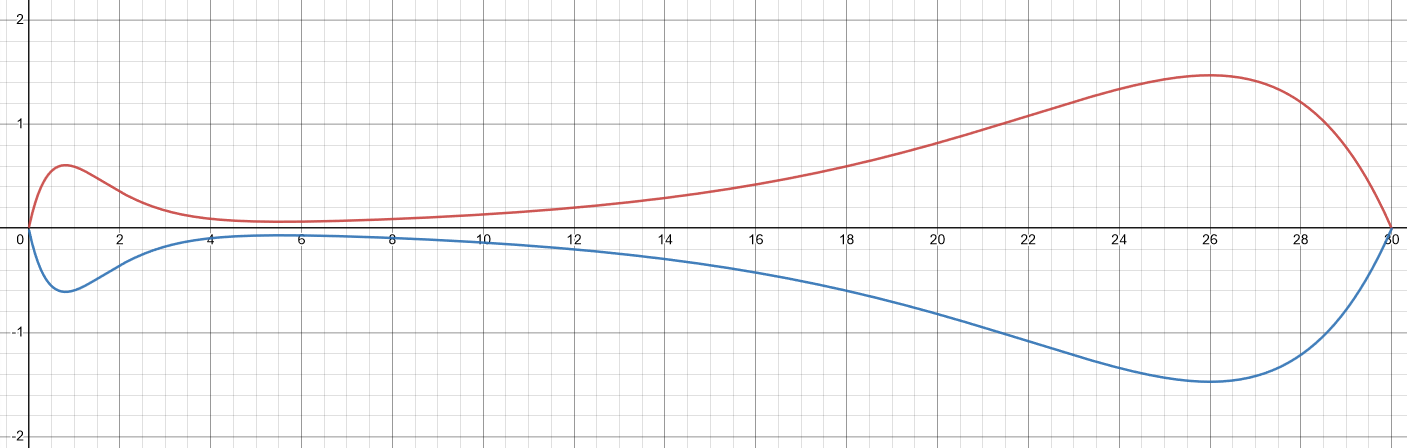
\includegraphics[width=.8\textwidth]{images/6-3-7.png}
    
    \begin{red}
    I mean, sure. It's a little pointy at the end and a little narrow in the handle but it's not terrible.
    \end{red}
    
    \item Let $x$ and $y$ be measured in inches. Find the total volume of the baseball bat generated by revolving the given curve about the $x$-axis. Include units on your answer.
    
    \begin{red}
    We should certainly slice vertically, and then our rectangles will revolve into disks. Therefore, the volume is given by
    \[V = \int_{x=0}^{x=30} \pi [f(x)]^2\ dx = \int_{x=0}^{x=30} \pi [2xe^{-1.25x} + (30-x) e^{-0.25(30-x)}]^2\ dx \approx 52.1 \text{ in}^3 \]
    (Thanks, Wolfram$\mid$Alpha!)
    \end{red}
    
    \item Suppose that the baseball bat has constant weight density, and that the weight density is $0.6$ ounces per cubic inch. Find the total weight of the bat whose volume you found in (b).
    
    \begin{red}
    Check the units: since our constant weight density is given in $\frac{\text{oz}}{\text{in}^3}$, and since our volume we just computed was in $\text{in}^3$, we just have to multiply:
    \[0.6\frac{\text{oz}}{\text{in}^3} \cdot 52.1 \text{ in}^3 \approx 31.26 \text{ oz}. \]
    \end{red}
    
    \item Because the baseball bat does not have constant cross-sectional area, we see that the amount of weight concentrated at a location $x$ along the bat is determined by the volume of a slice at location $x$. Explain why we can think about the function $\rho(x) = 0.6 \pi f(x)^2$ (where $f(x)$ is the function given at the start of the problem) as being the weight density function for how the weight of the baseball bat is distributed from $x=0$ to $x=30$.
    
    \begin{red}
    Look at a slice at a particular $x$-value. The \textbf{cross-sectional area} of that slice is $\pi r^2 = \pi f(x)^2$. (Which is not constant! A slice in the barrel of the bat will have bigger area than a slice in the handle.) So then if you multiply that cross-sectional area by the constant (volume) weight density $0.6\frac{\text{oz}}{\text{in}^3}$, well then by golly you get something with the units $\frac{\text{oz}}{\text{in}}$, which are completely sensible units for the (length) weight density function.
    \end{red}
    
    \item Compute the center of mass of the baseball bat.
    
    \begin{red}
    Now we have a $\rho(x)$ function that we can reasonably use our center-of-mass equation on. 
    
    Numerator: $\int_{x=0}^{x=30} x\cdot\rho(x)\ dx = \int_{x=0}^{x=30} x\cdot \left(0.6\pi [2xe^{-1.25x} + (30-x) e^{-0.25(30-x)}]^2\right)\ dx \approx 725.21$ oz$\cdot$in
    
    Denominator: $\int_{x=0}^{x=30} \rho(x)\ dx = 0.6 \int_{x=0}^{x=30} \pi[f(x)]^2\ dx$, which we've already found to be 31.26 oz.
    
    Center of mass: $\frac{725.21 \text{ oz}\cdot\text{in}}{31.26\text{ oz}} \approx 23.2$ in. (That's believable, looking at my picture.)
    \end{red}
    
    
\end{enumerate}

\end{enumerate}
\end{document}